%%%%%%%%%%%%%%%%%%%%%%%%%%%%%%%%%%%%%%%%%%%%%%%%
% E.Pinault-Bigeard - e.pinault-bigeard@upsti.fr
% http://s2i.pinault-bigeard.com
% CC BY-NC-SA 2.0 FR - http://creativecommons.org/licenses/by-nc-sa/2.0/fr/
%%%%%%%%%%%%%%%%%%%%%%%%%%%%%%%%%%%%%%%%%%%%%%%%
\documentclass[11pt]{article}
%%%%%%%%%%%%%%%%%%%%%%%%%%%%%%%%%%%%%%%%%%%%%%%%
% Package UPSTI_Document
%%%%%%%%%%%%%%%%%%%%%%%%%%%%%%%%%%%%%%%%%%%%%%%%
%%%%%%%%%%%%%%%%%%%%%%%%%%%%%%%%%%%%%%%%%%%%%%%%
% Package UPSTI_Document
%%%%%%%%%%%%%%%%%%%%%%%%%%%%%%%%%%%%%%%%%%%%%%%%
\usepackage{subcaption}
\usepackage[usenames, svgnames, dvipsnames]{xcolor}
\usepackage{UPSTI_Document}
\usepackage{pgfplots}
\usepackage{import}
\definecolor{darkspringgreen}{rgb}{0.09, 0.45, 0.27}

\newcommandx*{\dessinRepereFigGeo}[5][1=\vx{},2=\vy{},3=\vz{},4=,5=0]
	{
		\draw [->,very thick] (0,0) -- (1,0) ;
		\draw [->,very thick] (0,0) -- (0,1) ;
    \fill[white] (0,0) circle (0.13);
    \draw [->,very thick] (0,0) circle (0.13);
    \ifnumequal{#5}{0} {% z vers nous
      \fill[black] (0,0) circle (0.03);
      \draw [->,thick] (0,0) circle (0.04);
    }{% z vers la feuille
  		\begin{scope} [rotate=45]
  			\draw [-,thick] (0,-0.12) -- (0,0.12) ;
  			\draw [-,thick] (-0.12,0) -- (0.12,0) ;
  		\end{scope}
    }
		\draw [anchor=north west] (1.1,0) node {${#1}$};
		\draw [anchor=south west] (0,1.1) node {${#2}$};
		\draw [anchor=north east] (-0.1,0) node {${#3}$};
		\draw [anchor=north west] (-0.1,-0.1) node {${#4}$};
	}

	\usepackage{array}
	\newcolumntype{L}[1]{>{\raggedright\let\newline\\\arraybackslash\hspace{0pt}}m{#1}}
	\newcolumntype{C}[1]{>{\centering\let\newline\\\arraybackslash\hspace{0pt}}m{#1}}
	\newcolumntype{R}[1]{>{\raggedleft\let\newline\\\arraybackslash\hspace{0pt}}m{#1}}

	\usepackage{pifont}% http://ctan.org/pkg/pifont
\newcommand{\cmark}{\color{green}\ding{51}}%
\newcommand{\xmark}{\color{red}\ding{55}}%
\newcommand{\fmark}{\ding{229}}%
\newcommand{\itemc}{\item[\cmark]}%
\newcommand{\itemx}{\item[\xmark]}%
\newcommand{\itemf}{\item[\fmark]}%


\usetikzlibrary[circuits.plc.ladder]            %     
\newlength{\ladderskip}\setlength{\ladderskip}{5\tikzcircuitssizeunit}%5\tikzcircuitssizeunit    = 355pt
\newlength{\ladderrungsep}
\setlength{\ladderrungsep}{.2\ladderskip}
\def\ladderrungend#1{\pgftransformyshift{-#1\ladderskip-\ladderrungsep}}

%---------------------------------%
% Paramètres du package
%---------------------------------%

% Version du document (pour la compilation)
% 1: Document prof
% 2: Document élève
% 3: Document à publier
\newcommand{\UPSTIidVersionDocument}{2}


% Classe
% 1: PTSI				6: PSI*			11: TSI2		16: Spé
% 2: PT	(par défaut)	7: MPSI			12: ATS
% 3: PT*				8: MP			13: PC
% 4: PCSI				9: MP*			14: PC*
% 5: PSI				10: TSI1		15: Sup
%\newcommand{\UPSTIidClasse}{2}



% Matière
% 1: S2I (par défaut)    2: IPT     3: TIPE
% 6: Vie au lycée
\newcommand{\UPSTIvariante}{5}
\newcommand{\UPSTIidMatiere}{0}
\newcommand{\UPSTIintituleMatiere}{Automatique}
\newcommand{\UPSTIsigleMatiere}{Autom}
% Type de document
% 0: Custom*				7: Fiche Métho de			14: Document Réponses
% 1: Cours (par défaut)		8: Fiche Synthèse    		15: Programme de colle
% 2: TD     				9: Formulaire
% 3: TP						10: Memo
% 4: Colle					11: Dossier Technique
% 5: DS						12: Dossier Ressource
% 6: DM						13: Concours Blanc
% * Si on met la valeur 0, il faut décommenter la ligne suivante:
%\newcommand{\UPSTItypeDocument}{Custom}
\newcommand{\UPSTIidTypeDocument}{1}

% Titre dans l'en-tête


% Titre dans l'en-tête

\newcommand{\UPSTIvariante}{5}

\newcommand{\UPSTItitreEnTete}{Automatisme industriel}
%\newcommand{\UPSTItitreEnTetePages}{}
\newcommand{\UPSTIsousTitreEnTete}{Introduction aux API}


% Titre
%\newcommand{\UPSTItitrePreambule}{Automatisme industriel}
\newcommand{\UPSTItitre}{La programmation d'un Automate Industriel}

% Durée de l'activité (pour DS, DM et TP)
\newcommand{\UPSTIduree}{3h30}

% Note de bas de première page
%\newcommand{\UPSTInoteBasDePremierePage}{Geoffrey Vaquette}
% Numéro (ajoute " n°1" après DS ou DM)
\newcommand{\UPSTInumero}{2}

% Numéro chapitre
%\newcommand{\UPSTInumeroChapitre}{1}

% En-tête customisé
%\newcommand{\UPSTIenTetePrincipalCustom}{UPSTIenTetePrincipalCustom}

% Message sous le titre
%\newcommand{\UPSTImessage}{Message sous le titre}


% Référence au programme
%\newcommand{\UPSTIprogramme}{\EPBComp \EPBCompP{B1-02}, \EPBCompP{B2-49}, \EPBCompS{B2-50}, \EPBCompS{B2-51}, \EPBCompP{C1-07}, \EPBCompP{C1-08}}

% Si l'auteur n'est pas l'auteur par défaut
%\renewcommand{\UPSTIauteur}{WWOOOOOOWW}

% Si le document est réalisé au nom de l'équipe
%\newcommand{\UPSTIdocumentCollegial}{1}

% Source
\newcommand{\UPSTIsource}{G. Vaquette, H. Discours}

% Version du document
\newcommand{\UPSTInumeroVersion}{1.1}

%-----------------------------------------------
\UPSTIcompileVars		% "Compile" les variables
%%%%%%%%%%%%%%%%%%%%%%%%%%%%%%%%%%%%%%%%%%%%%%%%


%%%%%%%%%%%%%%%%%%%%%%%%%%%%%%%%%%%%%%%%%%%%%%%%
% Début du document
%%%%%%%%%%%%%%%%%%%%%%%%%%%%%%%%%%%%%%%%%%%%%%%%
\begin{document}
\UPSTIbuildPage

%\UPSTIobjectif{Durant cette activité, nous allons analyser une trame pour l'envoi d'informations sur une étiquette.}

\tableofcontents

\UPSTIremarque{Ce TP sera réalisé uniquement avec le logiciel « Logo Soft » en mode simulation, l’automate
ne sera pas raccordé.}
% \begin{figure}[bht]
%     \centering
%             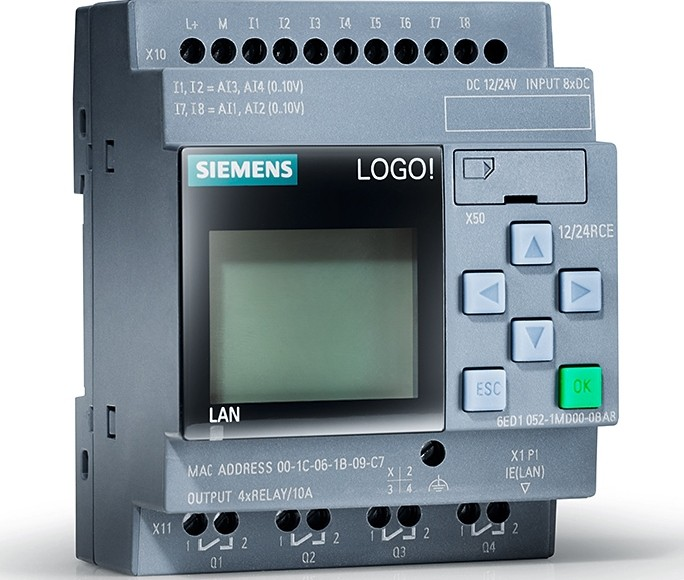
\includegraphics[width=.6\textwidth, height=.2\textheight,keepaspectratio]{images/logo-v8-siemens}
%             \caption{Automate Monobloc : Siemens LOGO}
%             \label{fig:logo}
% \end{figure}
\pagebreak
\section{Bascules RS}
Un bouton poussoir BP est placé sur l’entrée I1. Trois sorties, Q1, Q2 et Q3 commandent trois
voyants. Fonctionnement désiré :

\begin{itemize}
    \item Tous les voyants sont éteints au départ.
    \item L’appui sur BP provoque l’éclairement de Q1 (seulement).
    \item Le relâchement de BP provoque l’éclairement de Q2. Q1 reste allumé.
    \item Un nouvel appui sur BP provoque l’éclairement de Q3. Q2 et Q1restent allumés.
    \item Après le relâchement de BP, il n’y a plus que Q3 et Q2 d’allumés.
    \item Après un nouvel appui sur BP, il n’y a plus que Q3 d’allumé.
    \item Après le relâchement de BP, tous les voyants sont éteints. Le cycle peut redémarrer.
\end{itemize}

\begin{UPSTIactivite}
    \UPSTIquestion{Dessiner un chronogramme et un graphe d’état pour représenter le fonctionnement.}

    \UPSTIquestion{}

    On associe une bascule RS à la sortie Q1

    \begin{enumerate}
        \item Donner l’équation du set, noté S-Q1, en fonction de BP, Q2 et Q3
        \item Donner l’équation du reset, noté R-Q1, en fonction de BP, Q2 et Q3
    \end{enumerate}

    On associe une bascule RS à la sortie Q2
    \begin{enumerate}[resume]
        \item  Donner les équations des set et reset, notés S-Q2 et
        R-Q2 en fonction de BP, Q1 et Q3        
    \end{enumerate}

    On associe une bascule RS à la sortie Q3
    \begin{enumerate}[resume]
        \item Donner les équations des set et reset, notés S-Q3 et
        R-Q3 en fonction de BP, Q1 et Q2        
    \end{enumerate}
\end{UPSTIactivite}
\pagebreak
\begin{UPSTIactivite}
    \UPSTIquestion{Saisir dans Logo soft le programme correspondant, en logigramme. Pour une meilleure
    lisibilité, il est demandé de respecter l’organisation suivante :}
    \begin{center}
        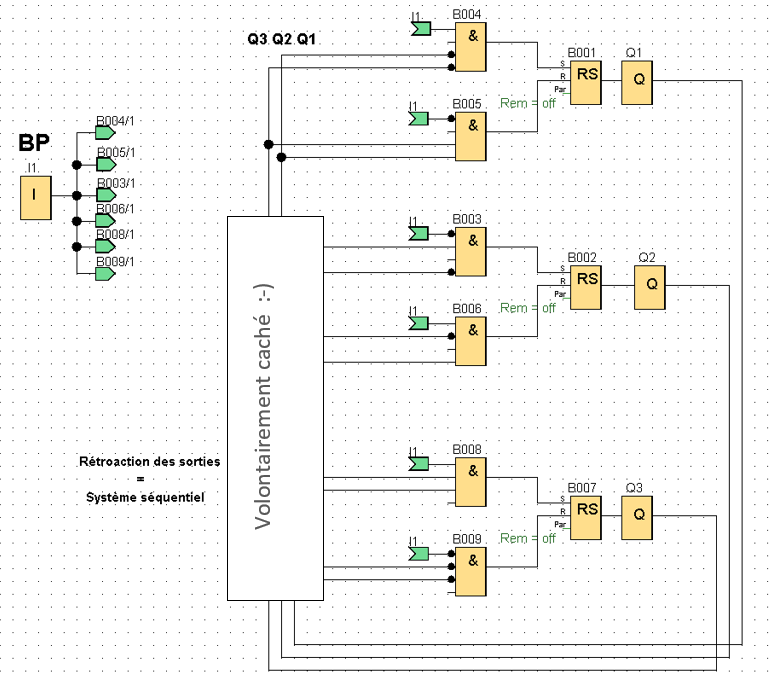
\includegraphics[width=.5\textwidth]{images/rs-activite2.png}
    \end{center}
    \textbf{Les bascules RS s'appellent \textit{Relais à automaintien} dans la bibliothèque}
\end{UPSTIactivite}

\section{Bascules, temporisations et fronts}

A partir d’un bouton unique, on cherche à réaliser la séquence prédéfinie suivante :


\begin{itemize}
    \item Tout est éteint au départ.
    \item L’appui sur un bouton I1 allume en orange l’écran, qui reste allumé au relâchement du
    bouton.
    \item 2 secondes plus tard, l’écran passe en rouge automatiquement (penser à éteindre l'éclairage orange)
    \item 2 secondes plus tard il reste rouge et le voyant Q1 s’allume.
    \item Tout reste allumé jusqu’à l’appui sur un second bouton I2, qui remet à zéro la séquence.    
\end{itemize}

\begin{UPSTIactivite}
    \UPSTIquestion{En utilisant un \textit{retard à l'enclenchement} pour les temporisation, implémenter le comportement désiré.}

    \begin{minipage}{.6\textwidth}
        Attention, il est nécessaire d'utiliser le front montant de I1 au lieu de I1 directement. Pour cela, utiliser une porte AND avec détection de front : 
    \end{minipage}
    \begin{minipage}{.3\textwidth}
        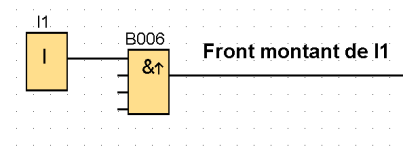
\includegraphics[width=\textwidth]{images/activite-frontAnd.png}
    \end{minipage}

    \UPSTIquestion{Que faut-il faire pour que la séquence soit lancée sur un front descendant du bouton ? }
    
\end{UPSTIactivite}

\pagebreak
\section{Compteurs}
\begin{UPSTIactivite}
    Réaliser le fonctionnement suivant : 

    \begin{center}
        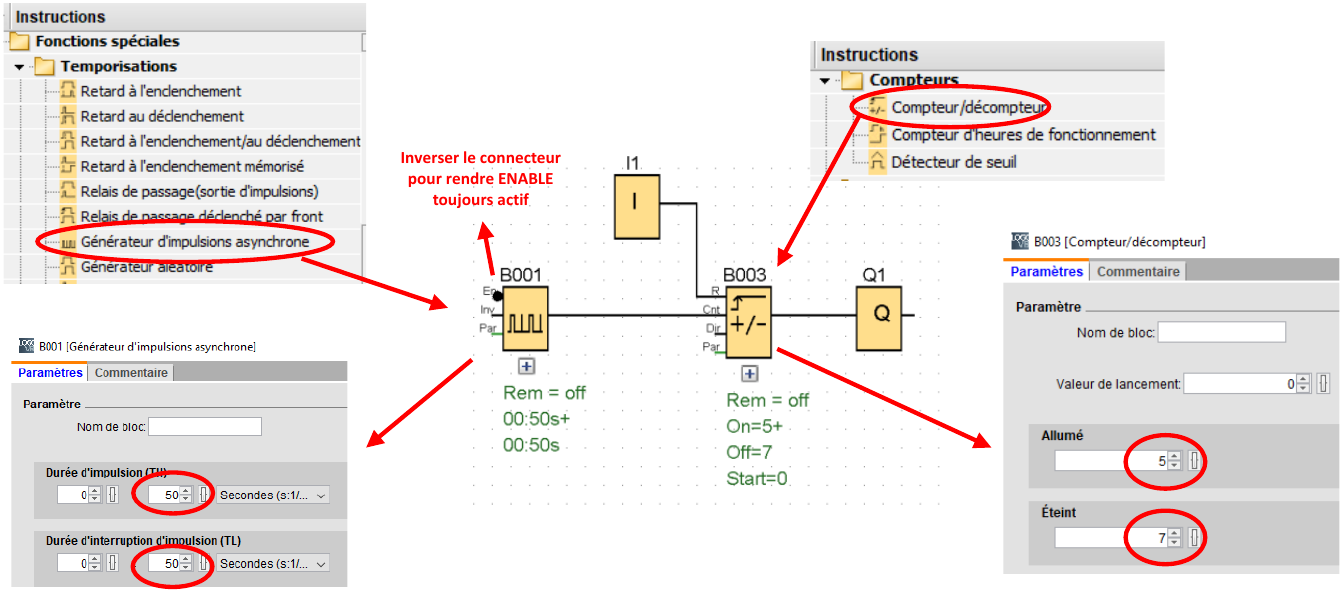
\includegraphics[width=\textwidth]{images/logigrammeCompteur.png}
    \end{center}

    \UPSTIquestion{Simuler le fonctionnement et expliquer le comportement des différents éléments.}
\end{UPSTIactivite}
\pagebreak
\begin{UPSTIactivite}
    Parfois sur certains appareils électroniques, on trouve une LED qui clignote pour signaler un
état. Et pour éviter de câbler plusieurs LEDs, pour signaler différents états, c’est le nombre de
clignotements sur une période donnée, qui permet de donner plusieurs informations.

Par exemple en choisissant une durée de 10 secondes :

\begin{minipage}{.3\textwidth}
    Pour une impulsion : 
\end{minipage}
\begin{minipage}{.6\textwidth}
    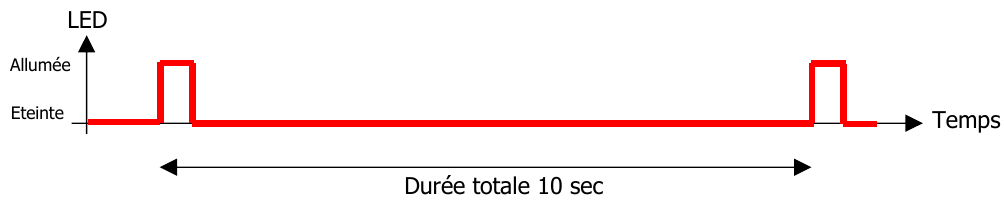
\includegraphics[width=\textwidth]{images/chrono_un_bip.png}
\end{minipage}

\begin{minipage}{.3\textwidth}
    Pour deux impulsions : 
\end{minipage}
\begin{minipage}{.6\textwidth}
    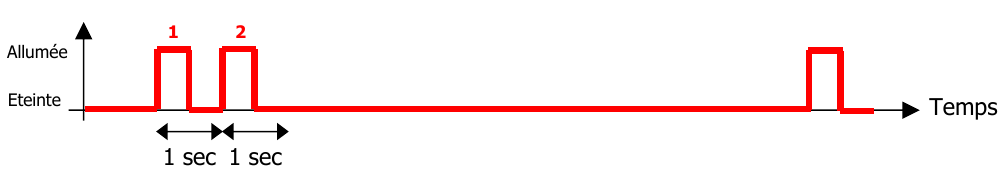
\includegraphics[width=\textwidth]{images/chrono_deux_bips.png}
\end{minipage}


Pour coder ce fonctionnement, commencer avec le logigramme ci-dessous : 

\begin{center}
    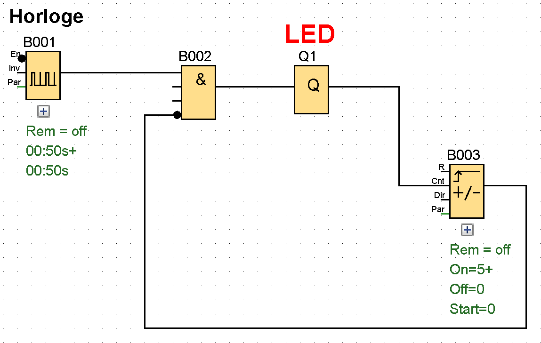
\includegraphics[width=.4\textwidth]{images/compteur_1.png}
\end{center}

Tester le fonctionnement 

\UPSTIquestion{Comment se comporte le compteur ?}

    Avec ce système, on peut observer une minuscule impulsion lorsque la valeur
voulue est atteinte. Ce phénomène, appelé « Glitch » en électronique, n’est pas recommandé.

\UPSTIquestion{Implémenter l'amélioration suivante, tester et expliquer}
\begin{center}
    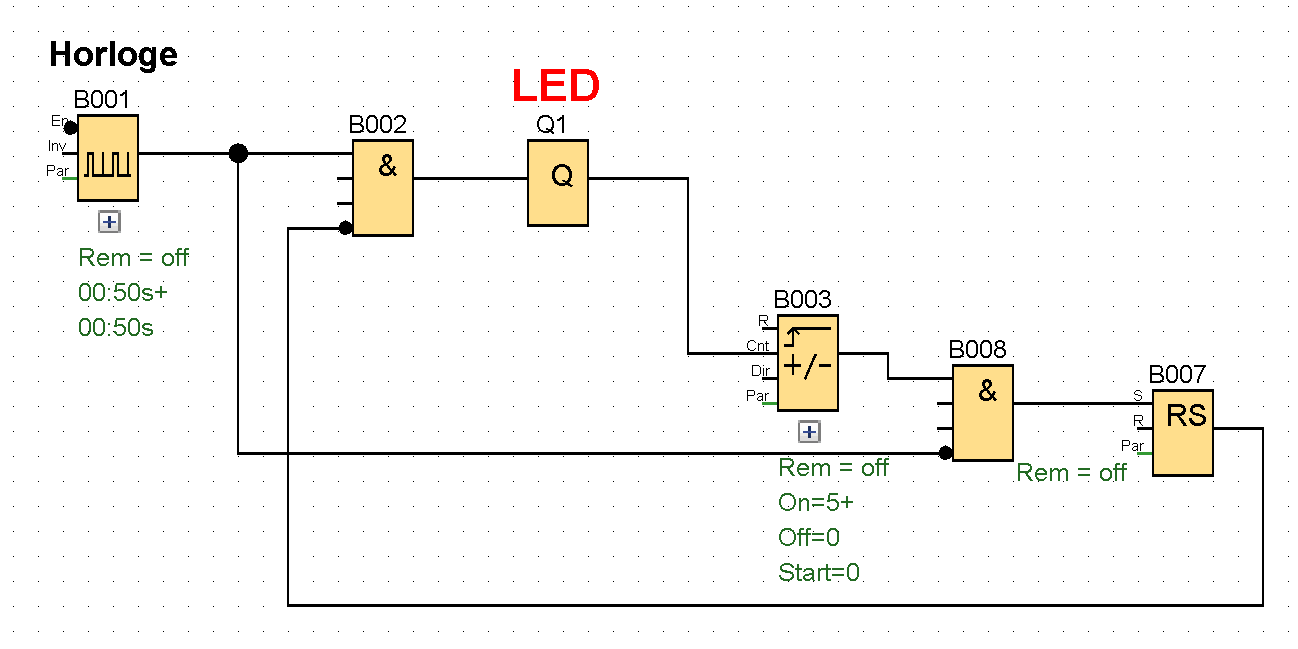
\includegraphics[width=.5\textwidth]{images/compteur_2.png}
\end{center}

On ajoute ensuite un second compteur pour que le fonctionnement recommence après 10 itération. 

\UPSTIquestion{Il manque un fil à ajouter sur la figure suivante, implémenter ce circuit en l'ajoutant}

\begin{center}
    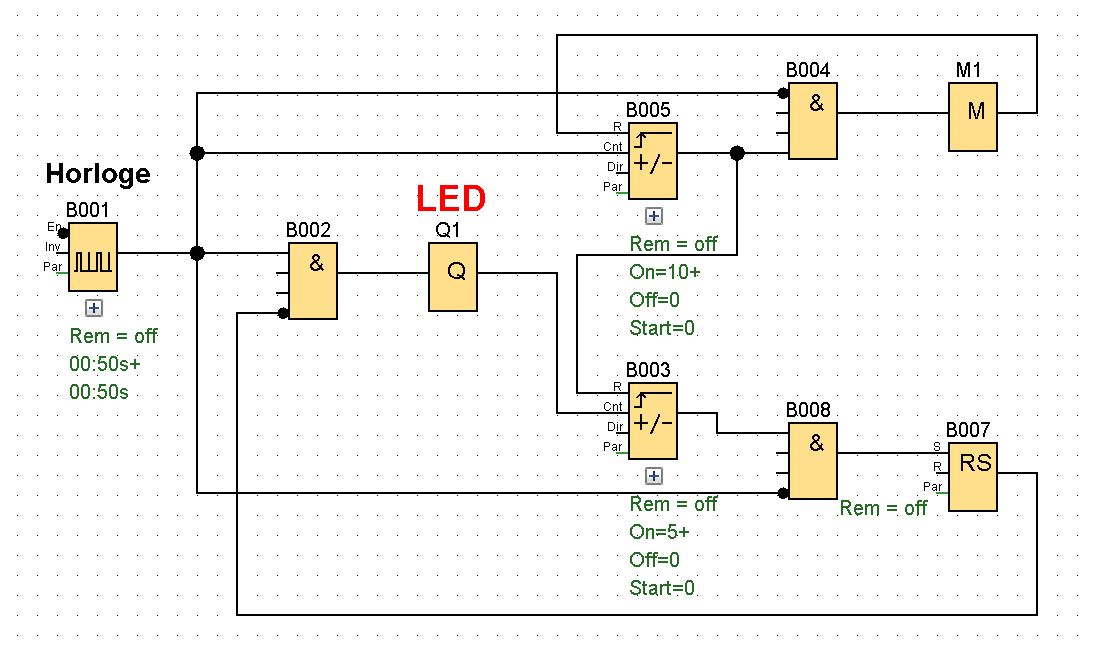
\includegraphics[width=.5\textwidth]{images/compteur_3.png}
\end{center}

\textbf{Faire valider par l'enseignant}
\end{UPSTIactivite}
\pagebreak
\section{Exercice de synthèse}
\begin{center}
    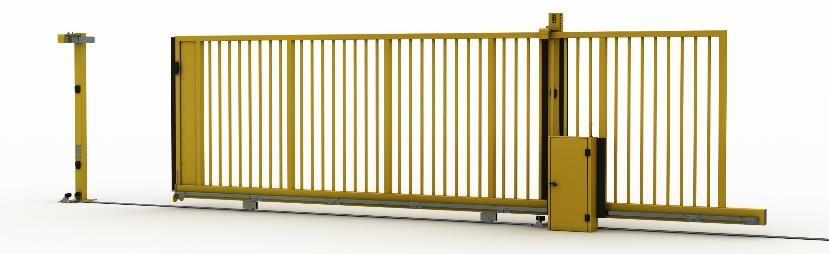
\includegraphics[width=.6\textwidth]{images/portail.jpg}
\end{center}

Soit un portail coulissant avec le comportement suivant : 
\begin{itemize}
    \item Un appui sur bouton I1 provoque l’ouverture (utiliser la sortie Q1 comme équivalent du moteur à l’ouverture) et faire afficher « OUVERTURE » sur l’écran du Logo.
    \item En fin de course, simulée avec le bouton I2, le moteur s’arrête.
    Au bout de 3 secondes, la sortie Q2 s’active (pour simuler le moteur à la fermeture).
    \item Faire afficher « FERMETURE » sur l’écran du Logo.
    \item En fin de course, simulée avec le bouton I3, le moteur s’arrête.
    Le système est alors prêt à recommencer un cycle.
\end{itemize}
\begin{UPSTIactivite}
    
    \UPSTIquestion{Mettre au point un programme pour réaliser la commande du portail coulissant.}
    \UPSTIquestion{Ajouter un compteur de cycles, qui :} 
    
    \begin{itemize}
        \item Au bout d’un certain nombre (prendre par exemple 3 pour les essais), affiche « MAINTENANCE CONSEILLEE ». 
        \item Lorsqu’une valeur max est atteinte
        (par exemple 5), cela interdit le lancement d’un nouveau cycle et affiche « MAINTENANCE
        OBLIGATOIRE », sur fond rouge.
    \end{itemize}
    
\end{UPSTIactivite}


\end{document}
